\begin{figure}
\begin{center}
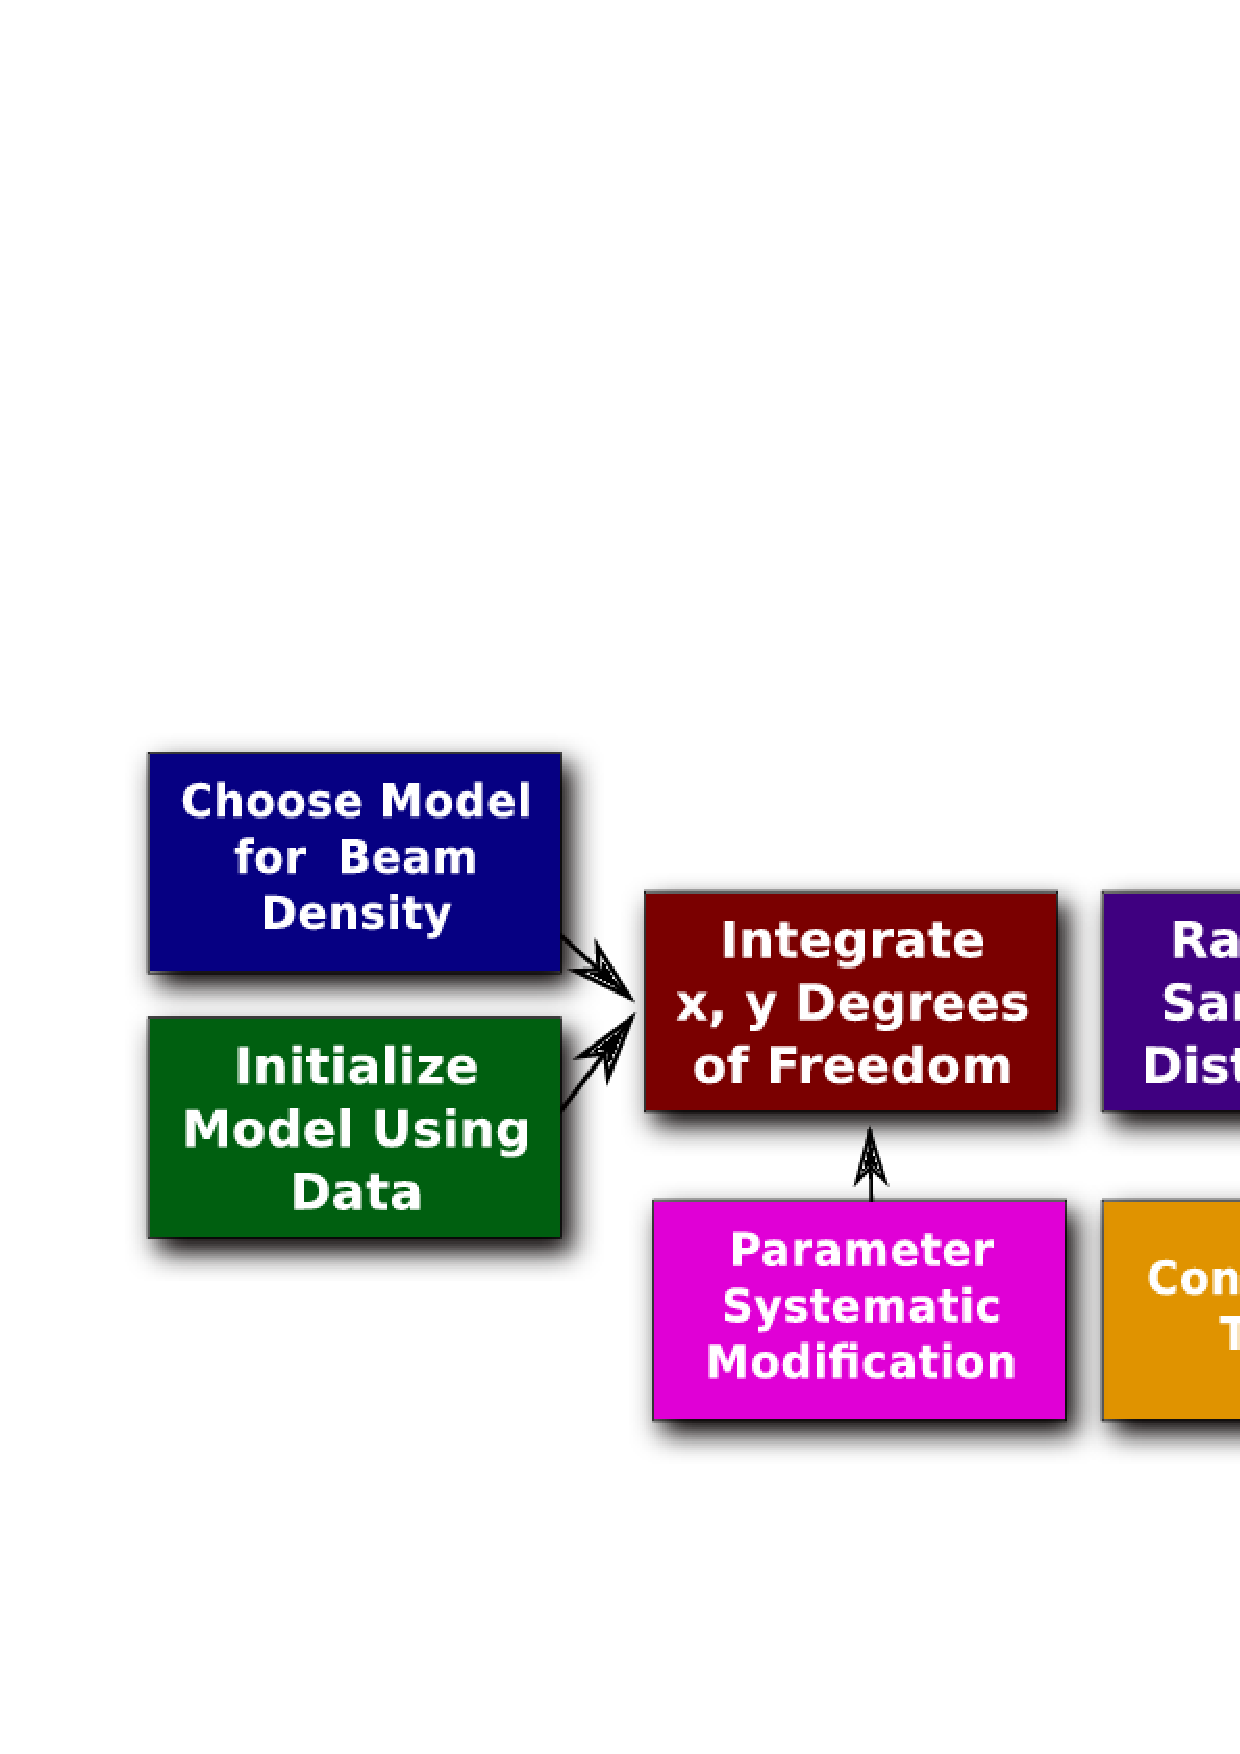
\includegraphics[width=\linewidth,height=\textheight,keepaspectratio]{../HourglassCorrection/figs/simulation_flow}
\caption{
Here we see the schematic overview of the simulation. Each box represents a
distinct step we take in the modeling or numeric integration of the luminosity.
Because we use numeric methods for solving the luminosity integral, we do not
have easy access to regression methods such as gradient-descent. Instead we
start matching the zdc z-vertex profile with the simulated profile, and then
vary the configuration parameters over reasonable ranges, choosing the result
which minimizes the difference between the distributions.
}
\label{fig:simulation_flow}
\end{center}
\end{figure}
